%!TEX root = ../../secondYearReport.tex

% 0.48 man.months for UPMC on T2.4,  

Within T2.4, Inria, TUD and UPMC participated in analysing the dataset of the EDHHI experiments\footnote{\url{http://www.loria.fr/~sivaldi/edhhi.htm}} where healthy adults (18-65 years old) interact physically with the iCub (see  Fig.~\ref{fig:eddhi_picture}). The analysed data include tactile data from the forearm skin and contact forces, estimated by the iDyn modules developed in WP1. The preliminary analysis shows that people, on average, learn quickly how to interact with the robot and move its arms: across three trials, the exchanged forces are smaller and the contacts more precise. Currently, Inria is coupling the analysis of tactile and force signals with individual factors and social signals exchanged by the two peers.

\begin{wrapfigure}{R}{0.5\textwidth}
  \begin{center}
    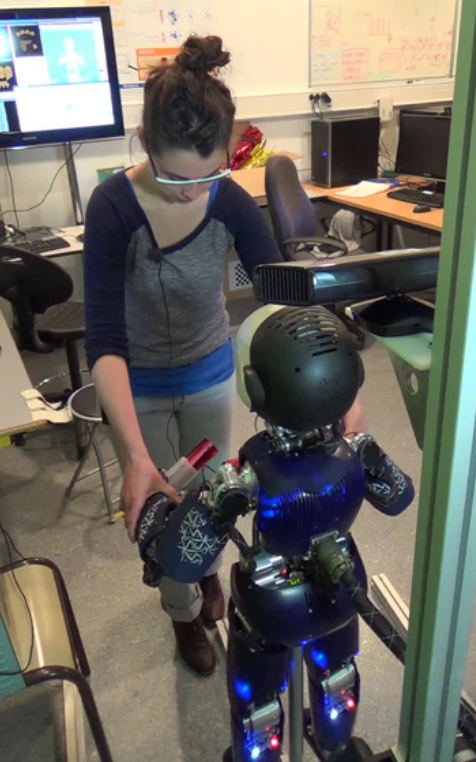
\includegraphics[width=0.48\textwidth]{pics_UPMC/eddhi_illustration}
  \end{center}
  \caption{View of a physical interaction between a human and the iCub robot.}
 \label{fig:eddhi_picture}
\end{wrapfigure}

